\documentclass[11pt]{article}
\usepackage{geometry,marginnote} % Pour passer au format A4
\geometry{hmargin=1cm, vmargin=1cm} % 

% Page et encodage
\usepackage[T1]{fontenc} % Use 8-bit encoding that has 256 glyphs
\usepackage[english,french]{babel} % Français et anglais
\usepackage[utf8]{inputenc} 

\usepackage{lmodern}
\setlength\parindent{0pt}

% Graphiques
\usepackage{graphicx,float,grffile}
\usepackage{pst-eucl, pst-plot,units} 

% Maths et divers
\usepackage{amsmath,amsfonts,amssymb,amsthm,verbatim}
\usepackage{multicol,enumitem,url,eurosym,gensymb}
\DeclareUnicodeCharacter{20AC}{\euro}

% Sections
\usepackage{sectsty} % Allows customizing section commands
\allsectionsfont{\centering \normalfont\scshape}

% Tête et pied de page

\usepackage{fancyhdr} 
\pagestyle{fancyplain} 

\fancyhead{} % No page header
\fancyfoot{}

\renewcommand{\headrulewidth}{0pt} % Remove header underlines
\renewcommand{\footrulewidth}{0pt} % Remove footer underlines

\newcommand{\horrule}[1]{\rule{\linewidth}{#1}} % Create horizontal rule command with 1 argument of height

%----------------------------------------------------------------------------------------
%   Début du document
%----------------------------------------------------------------------------------------

\begin{document}

\setlength{\columnseprule}{1pt}

\horrule{2px}
\section*{Chapitre 1 - Calculer et rédiger des calculs - \texttt{(T)}}
\horrule{2px}

L'objectif de ce chapitre est de savoir \textbf{rédiger des calculs}...

\section*{1 - Addition, Soustraction, Multiplication et Division}

On commence avec le cas simple de deux nombres et une seule opération. Certains calculs simples doivent savoir se faire de tête sans perdre de temps. La calculatrice doit également savoir être manipulée.

Une remarque de vocabulaire :

\begin{align*}
& 2 + 3 = 3 + 2 = 5 \\
& 3 \times 5 = 5 \times 3 = 15
\end{align*}

\reversemarginpar\marginnote{$\Box \Box$}
Les opérations + et $\times$ sont \textbf{commutatives}. L'ordre des nombres n'a pas d'importance. 


\begin{minipage}[t]{0.5\textwidth}\begin{align*}
10 - 6 &= 4\\
6 - 10 &= ... = -6 \text{ n'est pas égale à 4 !}
\end{align*}\end{minipage}
\begin{minipage}[t]{0.5\textwidth}\begin{align*}
10 \div 2 &= 5\\
2 \div 10 &= 0,2 \text{ n'est pas égale à 5 !}
\end{align*}\end{minipage}

\reversemarginpar\marginnote{$\Box \Box$}
Les opérations - et $\div$ ne sont pas commutatives. L'ordre des nombres dans l'opération est importance. 
On étudiera le cas : 6 - 10 dans \textbf{le chapitre 9}.

\section*{2 - Priorité de calculs}

Il y a des règles, des priorités de calculs qui sont à connaître s'il y a plusieurs opérations dans un calcul. 

\begin{center}
\reversemarginpar\marginnote{$\Box \Box$}
\reversemarginpar\marginnote{$\Box \Box$}[0.3cm]
    \fbox{\textbf{On commence avec les multiplications et les divisions.}} \\
\end{center} \vspace{-1cm}


\begin{minipage}[t]{0.5\textwidth}

\begin{align*}
1 + 2 \times 3 &= 1 + 6 \\
               &= 7
\end{align*}

\end{minipage}\begin{minipage}[t]{0.5\textwidth}

\begin{align*}
1 + 2 \times 3 &= 3 \times 3 \\
               &= 9
\end{align*}

\end{minipage}

\begin{minipage}[t]{0.5\textwidth}

\begin{align*}
12 \div 2 + 1 &= 6 + 2 \\
              &= 8
\end{align*}

\end{minipage}\begin{minipage}[t]{0.5\textwidth}

\begin{align*}
12 \div 2 + 1 &= 12 + 3 \\
              &= 4
\end{align*}

\end{minipage}

Le cas des opérations non commutatives : $-$ et $\div$ peut aussi poser problème... \\

\begin{center}
    \reversemarginpar\marginnote{$\Box \Box$}
    \fbox{\textbf{On fait plutôt les opérations de gauche à droite.}}
\end{center}  \vspace{-1cm}

\begin{minipage}[t]{0.5\textwidth}

\begin{align*}
24 \div 4 \div 2 &= 6 \div 2 \\
                 &= 3
\end{align*}

\end{minipage}\begin{minipage}[t]{0.5\textwidth}

\begin{align*}
24 \div 4 \div 2 &= 24 \div 2 \\
                 &= 12
\end{align*}

\end{minipage}

\begin{minipage}[t]{0.5\textwidth}

\begin{align*}
28 -  10 - 8 &= 18 - 8 \\
             &= 10
\end{align*}

\end{minipage}\begin{minipage}[t]{0.5\textwidth}

\begin{align*}
28 -  10 - 8 &= 28 - 2  \\
             &= 26
\end{align*}

\end{minipage}

\begin{center}
\reversemarginpar\marginnote{$\Box \Box$}
    \fbox{\textbf{Les calculs dans les parenthèses doivent être fait en premier...}} et peuvent parfois se faire en même temps.
\end{center}  \vspace{-1cm}

\begin{align*}
(2 +  10) \times 3 - (4 +2) &= 12 \times 3 - 6  \\
                            &= 36 - 6 \\
                            &= 30
\end{align*}

\newpage
\textbf{Remarque} : \\
\textit{Attention, toutes les calculatrices ne donnent pas toujours les mêmes résultats} : $8 \div 2(2+2) =$ 16 (TI) ou 1 (Casio)

\begin{minipage}[t]{0.5\textwidth}
  \begin{figure}[H]
        \centering
        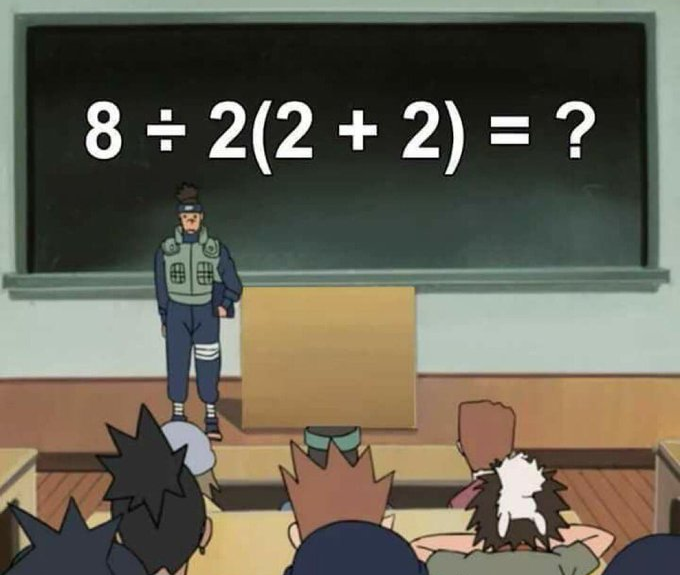
\includegraphics[width=0.7\linewidth]{5x1-calculer-et-rediger-des-calculs/naruto.png}
  \end{figure}
\end{minipage}
\begin{minipage}[t]{0.5\textwidth}
  \begin{figure}[H]
        \centering
        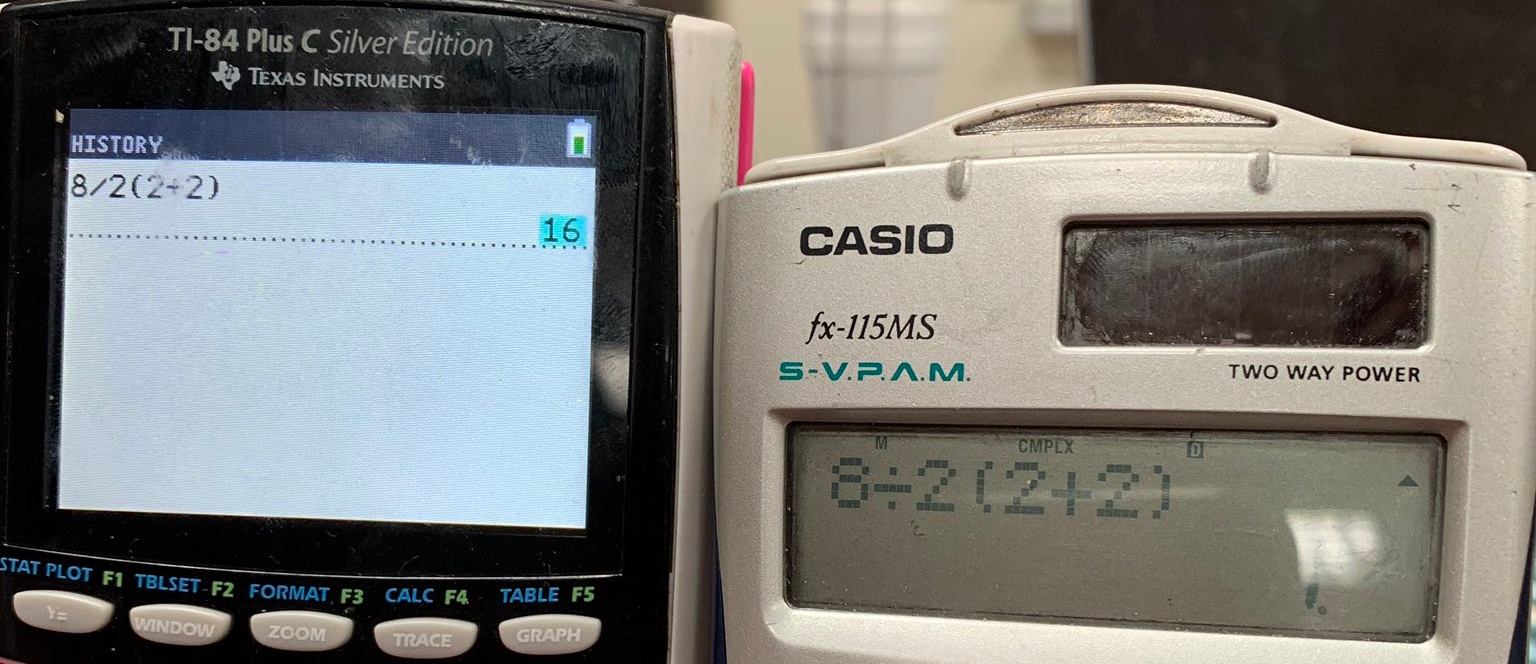
\includegraphics[width=\linewidth]{5x1-calculer-et-rediger-des-calculs/calc.png}
  \end{figure}
... cela veut dire que le calcul est mal écrit ...
\end{minipage}


\section*{3 - Calculer astucieusement}

Il est possible d'ête \textbf{malin} quand on fait des calculs. Il faut faire attention à bien respecter les règles de calculs...

\begin{minipage}[t]{0.33\textwidth}
\begin{align*}
25 + 7 + 75 &= 100 + 7  \\
            &= 107
\end{align*}

\end{minipage}
\begin{minipage}[t]{0.33\textwidth}

\begin{align*}
102 \times 6 &= 600 + 2 \times 6 \\
             &= 600 + 12 \\
             &= 612
\end{align*}

\end{minipage}
\begin{minipage}[t]{0.33\textwidth}

\begin{align*}
5 \times 7 \times 2 &= 10 \times 7 \\
                    &= 70
\end{align*}
\end{minipage}

\section*{4 - Convention d'écriture}

On essaye de remarquer comment j'ai rédigé mes calculs. On appelle cette compétence \textbf{communiquer}.

\begin{center}\reversemarginpar\marginnote{$\Box \Box$}
\reversemarginpar\marginnote{$\Box \Box$}[0.3cm]
\reversemarginpar\marginnote{$\Box \Box$}[0.6cm]
\reversemarginpar\marginnote{$\Box \Box$}[0.9cm]
\fbox{\begin{minipage}{0.6\textwidth}{\bfseries 
    \begin{itemize}
    \item Il faut écrire des étapes.
    \item Il faut passer à la ligne à chaque calcul.
    \item On aligne chaque signe égal.
    \item (On souligne le résultat.)
    \end{itemize}}
\end{minipage}}\end{center}

\textbf{On a le droit à la calculatrice. Toujours. Elle est personnelle et individuelle. Il faut quand même rédiger.}

\newpage

\section*{5 - Répondre à un problème}

Parfois les exercices de type problème ne donnent pas directement le calcul à faire. Il faut d'abord créer l'expression. On appelle cette compétence \textbf{Modéliser}.\\

\textsc{\textbf{Exercice} : Pour la rentrée, j'achète une règle à 1,20€, trois crayons à papiers à 1,10€ l'unité et deux 4-couleurs à 2,50€.} \newline
\textsc{Calculer le prix à payer en caisse ?}\\

\textsc{\textbf{Correction} :}\\

Calcul du prix à payer :
\begin{align*}
1,20 + 3 \times 1,10 + 2 \times 2,50 &= 1,20 + 3,30 + 5 \\
                                     &= 9,5
\end{align*}

Le prix a payer en caisse est 9,50€.



\begin{center}
\reversemarginpar\marginnote{$\Box \Box$}
\reversemarginpar\marginnote{$\Box \Box$}[0.3cm]
\reversemarginpar\marginnote{$\Box \Box$}[0.6cm]
\fbox{\begin{minipage}{0.6\textwidth}{\bfseries 
    \begin{itemize}
    \item Il faut dire quel calcul on fait.
    \item Il faut créer une expression à calculer. (Modéliser)
    \item Il faut rédiger le calcul avec les étapes.
    \item Il faut faire une phrase réponse.
    \end{itemize}}
\end{minipage}}
\end{center}


\section*{6 - Répondre à un programme de calcul}

Cet exercice particulier mérite sa place dans le cours. C'est un programme de calcul. On fait des calculs les uns à la suite des autres. Créer l'expression est un peu plus dur et demande parfois de rajouter des parenthèses. Il faut aussi connaitre un peu de vocabulaire en français ! Retrancher, Soustraire Ajouter, Additionner, Prendre le double... \\

\textbf{Exercice} : 

\begin{center}\fbox{\begin{minipage}{0.4\textwidth}
  {\fontfamily{lmtt}\selectfont 
    \begin{itemize}
      \item Prendre le nombre de départ.
      \item Ajouter 10.
      \item multiplier par 4.
      \item Retrancher 40.
    \end{itemize}
  }
\end{minipage}}\end{center}

\textsc{Faire le programme de calcul avec : 0, 2, 100.} \\

\textbf{Correction} :

\begin{minipage}{0.3\textwidth}

\begin{align*}
& 0 \\
& 0 + 10 = 10 \\
& 10 \times 4 = 40\\
& 40 - 40 = 0
\end{align*}

\end{minipage}\begin{minipage}{0.3\textwidth}

\begin{align*}
& 2 \\
& 2 + 10 = 12 \\
& 12 \times 4 = 48\\
& 48 - 40 = 8
\end{align*}

\end{minipage}\begin{minipage}{0.3\textwidth}

\begin{align*}
& 100 \\
& 100 + 10 = 110 \\
& 110 \times 4 = 440\\
& 440 - 40 = 400
\end{align*}

\end{minipage}

\begin{center}\reversemarginpar\marginnote{$\Box \Box$}
\fbox{\begin{minipage}{0.6\textwidth}{\bfseries 

    \begin{itemize}
    \item Il faut écrire le nombre de départ.
    \item Il faut aligner les lignes de calcul.
    \item (On souligne le résultat.)
    \end{itemize}}

\end{minipage}}
\end{center}

\end{document}
